\chapter{Machine Learning} \label{chp:machinelearning}
\epigraph{Great quote.}{Author}
\begin{figure}[H]
	\centering
	
\includegraphics[scale=0.4]{Images/example.png}
	\caption{Caption}
\end{figure}

\iffalse
Parameter estimation is a large part of science, because we are often not able to measure things directly. For instance, when Millikan in ... performed his famous electron charge experiment or when we estimate Sun's mass.
\fi 

The use of the term \textit{machine learning} has exploded over the past years, and sometimes it sounds like it is a totally new field. However, the truth is that many of the methods we use are quite old, where for instance \textit{linear regression} was known early in the 19th century. \cite{legendre_nouvelles_1805}\cite{gauss_theoria_1809} Those methods have just recently been taken under the \textit{machine learning} umbrella, which is one of the reasons why the term is mentioned so often. As the UiO professor Anne Solberg pointed out during one of her lectures\\

''\textit{In the early 1990's I was working a lot with machine learning, but at that time we called it pattern recognition and regression...}''\\

Another reason why machine learning has an increasingly popularity is that some of the algorithms have been significantly improved. \textit{Convolutional Neural Networks} (CNNs) are now as good as humans when it comes to object recognition in images, and \textit{Long Short-Term Memory Recurrent Neural Networks} (LSTM RNNs) has improved voice recognition. 

We can conclude that Machine learning includes all methods where we want to fit models to data sets, and pattern recognition and regression are clearly some of those methods. In both cases we have concrete targets for the training, and the training is therefore called supervised training. In other cases we do not have targets, but want to train our model based on a probability distribution or so, which is called unsupervised learning.

\section{Supervised Learning}
In supervised learning methods, the input data has known targets such that we can fit a model to give the correct outputs. Linear regression is perhaps the most intuitive example on this, where we want to find the line that fits some data points in the best possible way. This corresponds to a neural network without any hidden layer, but when we add more layers the model is no longer linear and it all gets more complex. For simple classification tasks, logistic regression can be used. 

\subsection{Linear regression}
In linear regression, the dependent variable $y_i$ is a linear combination of the parameters, and for a dependent variable this can be written as
\begin{equation}
y_i=\sum_jX_{ij}\beta_j
\end{equation}
where $\beta_j$'s are the unknown parameters to be found. In principle, $X_{ij}$ can be an arbitrary function of the arguments $x_i$, but often one wants a polynomial model which corresponds to $X_{ij} = x_i^j$.

The three most commonly used linear regression methods are Ordinary Least Square (OLS) regression, Ridge regression and Lasso regression, where the former has the cost function
\begin{empheq}[box={\mybluebox[5pt]}]{equation}
	c(\vec{\beta})=\sum_{i=1}^{n}\Big(y_i-\beta_0-\sum_{j=1}^pX_{ij}\beta_j\Big)^2\qquad\qquad\qquad\text{OLS},
\end{empheq}
which is minimized when
\begin{equation}
\vec{\beta}=(\hat{X}^T\hat{X})^{-1}\hat{X}^T\vec{y}.
\end{equation}
Similarly, the Ridge cost function is
\begin{empheq}[box={\mybluebox[5pt]}]{equation}
	c(\vec{\beta})=\sum_{i=1}^{n}\Big(y_i-\beta_0-\sum_{j=1}^pX_{ij}\beta_j\Big)^2+\lambda\sum_{j=1}^p\beta_j^2\qquad\text{Ridge}
\end{empheq}
where $\lambda$ is called the penalty. This is minimized when
\begin{equation}
\vec{\beta}=(\hat{X}^T\hat{X}+\lambda I)^{-1}\hat{X}^T\vec{y},
\end{equation}
and finally the Lasso cost function is given by
\begin{empheq}[box={\mybluebox[5pt]}]{equation}
	c(\vec{\beta})=\sum_{i=1}^{n}\Big(y_i-\beta_0-\sum_{j=1}^pX_{ij}\beta_j\Big)^2+\lambda\sum_{j=1}^p\beta_j\qquad\text{Lasso}.
\end{empheq}

\subsection{Logistic regression}
Despite its name, logistic regression is not a fitting tool, but rather a classification tool. Traditionally, the perceptron model was used for 'hard classification', which sets the outputs directly to binary values. However, often we are interested in the probability of a given category, which means that we need a continuous \textit{activation function}. Logistic regression can, like linear regression, be considered as a function where coefficients are adjusted with the intention to minimize the error. Here, the coefficients are called \textit{weights}. The process goes like this: The inputs are multiplied by several weights, and by adjusting those weights the model can classify every \textit{linear classification problem}. A drawing of the perceptron is found in figure (\ref{fig:single_perceptron}).

\begin{figure} [H]
	\centering
	\begin{tikzpicture}
	\node[functions] (center) {};
	\node[below of=center,font=\scriptsize,text width=4em] {Activation function};
	\draw[thick] (0.5em,0.5em) -- (0,0.5em) -- (0,-0.5em) -- (-0.5em,-0.5em);
	\draw (0em,0.75em) -- (0em,-0.75em);
	\draw (0.75em,0em) -- (-0.75em,0em);
	\node[right of=center] (right) {};
	\path[draw,->] (center) -- (right);
	\node[functions,left=3em of center] (left) {$\sum$};
	\path[draw,->] (left) -- (center);
	\node[weights,left=3em of left] (2) {$w_2$} -- (2) node[input,left of=2] (l2) {$x_2$};
	\path[draw,->] (l2) -- (2);
	\path[draw,->] (2) -- (left);
	\node[below of=2] (dots) {$\vdots$} -- (dots) node[left of=dots] (ldots) {$\vdots$};
	\node[weights,below of=dots] (n) {$w_n$} -- (n) node[input,left of=n] (ln) {$x_n$};
	\path[draw,->] (ln) -- (n);
	\path[draw,->] (n) -- (left);
	\node[weights,above of=2] (1) {$w_1$} -- (1) node[input,left of=1] (l1) {$x_1$};
	\path[draw,->] (l1) -- (1);
	\path[draw,->] (1) -- (left);
	\node[weights,above of=1] (0) {$b$} -- (0) node[input,left of=0] (l0) {$B$};
	\node[right of=0,font=\scriptsize] {BIAS};
	\path[draw,->] (l0) -- (0);
	\path[draw,->] (0) -- (left);
	\node[below of=ln,font=\scriptsize] {inputs};
	\node[below of=n,font=\scriptsize] {weights};
	\end{tikzpicture}
	\caption{Logistic regression model with $n$ inputs.}
	\label{fig:single_perceptron}
\end{figure}
In logistic regression, we usually have one binary output node for each class, but for two categories one output node is sufficient, which can be fired or not fired. 

Initially, one needs to train the perceptron such that it knows which outputs are correct, and for that one needs to know the outputs that correspond to the inputs. Every time the network is trained, the weights are adjusted such that the error is minimized.

The very first step is to calculate the initial outputs (forward phase), where the weights usually are set to small random numbers. Then the error is calculated, and the weights are updated to minimize the error (backward phase). So far so good.

\subsubsection{Forward phase}\label{sec:forward}
Let us look at it from a mathematical perspective, and calculate the net output. The net output seen from an output node is simply the sum of all the "arrows" that point towards the node, see figure (\ref{fig:single_perceptron}), where each "arrow" is given by the left-hand node multiplied with its respective weight. For example, the contribution from input node 2 to the output node follows from $X_2\cdot w_{2}$, and the total net output to the output $O$ is therefore
\begin{empheq}[box={\mybluebox[5pt]}]{equation}
	net = \sum_{i=1}^{I} x_i\cdot w_i + b\cdot 1.
	\label{eq:forward}
\end{empheq}
Just some notation remarks: $x_i$ is the value of input node $i$ and $w_{i}$ is the weight which connects input $i$ to the output. $b$ is the bias weight, which we will discuss later.

You might wonder why we talk about the net output all the time, do we have other outputs? If we look at the network mathematically, what we talk about as the net output should be our only output. Anyway, it turns out to be convenient mapping the net output to a final output using an activation function, which is explained further in section \ref{sec:sigmoid1}. The activation function, $f$, takes in the net output and gives the output, 
\begin{equation}
out = f(net).
\end{equation}
If not everything is clear right now, it is fine. We will discuss the most important concepts before we dive into the maths.

\subsubsection{BIAS}
As mentioned above, we use biases when calculating the outputs. The nodes, with value $B$, are called the bias nodes, and the weights, $b$, are called the bias weights. But why do we need those? 

Suppose we have two inputs of value zero, and one output which should not be zero (this could for instance be a NOR gate). Without the bias, we will not be able to get any other output than zero, and in fact the network would struggle to find the right weights even if the output had been zero. 

The bias value $B$ does not really matter since the network will adjust the bias weights with respect to it, and is usually set to 1 and ignored in the calculations. [2]

\subsubsection{Learning rate}
In principle, the weights could be updated without adding any learning rate ($\eta=1$), but this can in practice be problematic. It is easy to imagine that the outputs can be fluctuating around the targets without decreasing the error, which is not ideal, and a learning rate can be added to avoid this. The downside is that with a low learning rate the network needs more training to obtain the correct results (and it takes more time), so we need to find a balance. 

\subsubsection{Cost function}\label{sec:cost_function}
The cost function is what defines the error, and in logistic regression the cross-entropy function is a naturally choice. [3] It reads
\begin{empheq}[box={\mybluebox[5pt]}]{equation}
	c(\boldsymbol{W}) = -\sum_{i=1}^n\Big[y_i\log f(\boldsymbol{x}_i^T\boldsymbol{W})+(1-y_i)\log[1-f(\boldsymbol{x}_i^T\boldsymbol{W})]\Big]
	\label{eq:cross_entropy}
\end{empheq}
where $\bs{W}$ contains all weights, included the bias weight ($\bs{W}\equiv[b,\bs{W}]$), and similarly does $\bs{x}$ include the bias node, which is 1; $\bs{x}\equiv[1,\bs{x}]$. Further, the $f(x)$ is the activation function discussed in next section.

The cross-entropy function is derived from likelyhood function, which famously reads
\begin{equation}
p(y|x)=\hat{y}^y\cdot(1-\hat{y})^{1-y}.
\end{equation}
Working in the log space, we can define a log likelyhood function
\begin{align}
	\log\Big[p(y|x)\Big]&=\log\Big[\hat{y}^y\cdot(1-\hat{y})^{1-y}\Big]\\
	&=y\log\hat{y}+(1-y)\log(1-\hat{y})
\end{align}
which gives the log of the probability of obtaining $y$ given $x$. We want this quantity to increase then the cost function is decreased, so we define our cost function as the negative log likelyhood function. [7]

Additionally, including a regularization parameter $\lambda$ inspired by Ridge regression is often convenient, such that the cost function is
\begin{equation}
c(\bs{W})^+=c(\bs{W})+\lambda||\bs{W}||_2^2.
\end{equation}
We will later study how this regularization affects the classification accuracy. 

\subsubsection{Activation function}\label{sec:sigmoid1}
Above, we were talking about the activation function, which is used to activate the net output. In binary models, this is often just a step function firing when the net output is above a threshold. For continuous outputs, the logistic function given by
\begin{empheq}[box={\mybluebox[5pt]}]{equation}
	f(x)=\frac{1}{1+e^{-x}}.
	\label{eq:logistic}
\end{empheq}
is usually used in logistic regression to return a probability instead of a binary value. This function has a simple derivative, which is advantageous when calculating a large number of derivatives. As shown in section \ref{sec:sigmoid_der}, the derivative is simply
\begin{equation}
\frac{df(x)}{dx}=x(1-x).
\label{eq:logistic_der}
\end{equation}

$tanh(x)$ is another popular activation function in logistic regression, which more or less holds the same properties as the logistic function. 

\subsubsection{Backward phase}
Now all the tools for finding the outputs are in place, and we can calculate the error. If the outputs are larger than the targets (which are the exact results), the weights need to be reduced, and if the error is large the weights need to be adjusted a lot. The weight adjustment can be done by any minimization method, and we will look at a couple of gradient methods. To illustrate the point, we will stick to the \textbf{gradient descent} (GD) method in the calculations, even though other methods will be used later. The principle of GD is easy: each weight is "moved" in the direction of steepest slope,
\begin{empheq}[box={\mybluebox[5pt]}]{equation}
	\bs{w}^+= \bs{w} - \eta\cdot\frac{\partial c(\boldsymbol{w})}{\partial \bs{w}},
	\label{eq:w_update}
\end{empheq}
where $\eta$ is the learning rate and $c(\bs{w})$ is the cost function. We use the chain rule to simplify the derivative
\begin{equation}
\frac{\partial c(\bs{w})}{\partial \bs{w}} =\frac{\partial c(\bs{w})}{\partial out} \cdot\frac{\partial out}{\partial net} \cdot\frac{\partial net}{\partial \bs{w}}
\end{equation}
where the first is the derivative of the cost function with respect to the output. For the cross-entropy function, this is
\begin{equation}
\frac{\partial c(\bs{w})}{\partial out}=-\frac{y}{out}+\frac{1-y}{1-out}.
\end{equation}
Further, the second derivative is the derivative of the activation function with respect to the output, which is given in \eqref{eq:logistic_der}
\begin{equation}
\frac{\partial out}{\partial net}=out(1-out).
\end{equation}
The latter derivative is the derivative of the net output with respect to the weights, which is simply
\begin{equation}
\frac{\partial net}{\partial \bs{w}}=\bs{x}.
\end{equation}

If we now recall that $out=f(\bs{x}^T\bs{w})$, we can write 
\begin{equation}
\frac{\partial c(\bs{w})}{\partial \bs{w}}=[f(\bs{x}^T\bs{w})-\bs{y}]\bs{x}
\end{equation}
and obtain a weight update algorithm
\begin{empheq}[box={\mybluebox[5pt]}]{align}
	\bs{w}^+= \bs{w} - \eta\cdot[f(\bs{x}^T\bs{w})-\bs{y}]^T\bs{x}.
\end{empheq}
where the bias weight is included implicitly in $\bs{w}$ and the same applies for $\bs{x}$.

\subsection{Neural network} \label{sec:neural_network}
If you have understood logistic regression, understanding a neural network should not be a difficult task. According to  \textbf{the universal approximation theorem}, a neural network with only one hidden layer can approximate any continuous function. [8] However, often multiple layers are used since this tends to give fewer nodes in total. 

In figure \eqref{fig:neural_network}, a two-layer neural network (one hidden layer) is illustrated. It has some similarities with the logistic regression model in figure \eqref{fig:single_perceptron}, but a hidden layer and multiple outputs are added. In addition, the output is no longer probabilities and can take any number, which means that we do not need to use the logistic function on the outputs anymore.

\begin{figure} [H]
	\centering
	\begin{tikzpicture}
	
	% Define outputs
	\node[] (center) {};
	\node[input, above=0.3em of center] (o1) {$o_1$};
	\node[input, below=0.3em of center] (o2) {$o_2$};
	
	% Draw lines from output nodes
	\node[right of=o1] (righto1) {};
	\node[right of=o2] (righto2) {};
	\path[draw,->] (o1) -- (righto1);
	\path[draw,->] (o2) -- (righto2);
	
	% Hidden nodes
	\node[input,left=5em of center] (h3) {$h_3$};
	\node[input,above of=h3] (h2) {$h_2$};
	\node[input,above of=h2] (h1) {$h_1$};
	\node[input,below of=h3] (h4) {$h_4$};
	\node[input,below of=h4] (h5) {$h_5$};
	\node[input,above of=h1] (b2) {$b_2$};
	
	% Draw lines from hidden nodes
	\path[draw,->] (h1) -- (o1);
	\path[draw,->] (h2) -- (o1);
	\path[draw,->] (h3) -- (o1);
	\path[draw,->] (h4) -- (o1);
	\path[draw,->] (h5) -- (o1);
	\path[draw,->] (b2) -- (o1);
	
	\path[draw,->] (h1) -- (o2);
	\path[draw,->] (h2) -- (o2);
	\path[draw,->] (h3) -- (o2);
	\path[draw,->] (h4) -- (o2);
	\path[draw,->] (h5) -- (o2);
	\path[draw,->] (b2) -- (o2);
	
	% Define place left of left
	\node[input,left=5em of h3] (x2) {$x_2$};
	\node[input,above of=x2] (x1) {$x_1$};
	\node[input,below of=x2] (x3) {$x_3$};
	\node[input,above of=x1] (b1) {$b_1$};
	
	% Draw lines from input nodes
	\path[draw,->] (x1) -- (h1);
	\path[draw,->] (x1) -- (h2);
	\path[draw,->] (x1) -- (h3);
	\path[draw,->] (x1) -- (h4);
	\path[draw,->] (x1) -- (h5);
	
	\path[draw,->] (x2) -- (h1);
	\path[draw,->] (x2) -- (h2);
	\path[draw,->] (x2) -- (h3);
	\path[draw,->] (x2) -- (h4);
	\path[draw,->] (x2) -- (h5);
	
	\path[draw,->] (x3) -- (h1);
	\path[draw,->] (x3) -- (h2);
	\path[draw,->] (x3) -- (h3);
	\path[draw,->] (x3) -- (h4);
	\path[draw,->] (x3) -- (h5);
	
	\path[draw,->] (b1) -- (h1);
	\path[draw,->] (b1) -- (h2);
	\path[draw,->] (b1) -- (h3);
	\path[draw,->] (b1) -- (h4);
	\path[draw,->] (b1) -- (h5);
	
	% Draw lines towards input nodes
	\node[left of=x1] (leftx1) {};
	\node[left of=x2] (leftx2) {};
	\node[left of=x3] (leftx3) {};
	\path[draw,->] (leftx1) -- (x1);
	\path[draw,->] (leftx2) -- (x2);
	\path[draw,->] (leftx3) -- (x3);
	
	% Add some text
	\node[below=5.1em of x2,font=\scriptsize] {input};
	\node[below=5em of h3,font=\scriptsize] {hidden};
	\node[below=5.8em of center,font=\scriptsize] {output};
	\end{tikzpicture}
	\caption{Neural network with 3 input nodes, 5 hidden nodes and 2 output nodes, in addition to the bias nodes.}
	\label{fig:neural_network}
\end{figure}

Without a hidden layer, we have seen that the update of weights is quite straight forward. For a neural network consisting of multiple layers, the question is: how do we update the weights when we do not know the values of the hidden nodes? And how do we know which layer causing the error? This will be explained in section \ref{sec:backward}, where one of the most popular techniques for that is discussed. Before that we will generalize the forward phase presented in logistic regression.

\subsubsection{Forward phase}
In section \ref{sec:forward}, we saw how the output is found for a single perceptron. Since we only had one output node, the weights could be stored in an array. Generally, it is more practical to store the weights in matrices, since they will have indices related to both the node on left-hand side and the node on the right-hand side. For instance, the weight between input node $x_3$ and hidden node $h_5$ in figure \eqref{fig:neural_network} is usually labeled as $w_{35}$. Since we have two layers, we also need to denote which weight set it belongs to, which we will do by a superscript ($w_{35}\Rightarrow w_{35}^{(1)}$). In the same way, $\bs{W}^1$ is the matrix containing all $w_{ij}^{(1)}$, $\bs{x}$ is the vector containing all $x_i$'s and so on. We then find the net outputs at the hidden layer to be
\begin{empheq}{equation}
	net_{h,j} = \sum_{i=1}^{I} x_i\cdot w_{ij}^{(1)}=\bs{x}^T\bs{W}_j^{(1)}
	\label{eq:forward_hidden}
\end{empheq}
where the $\bs{x}$ and $\bs{W}^{(1)}$ again are understood to take the biases. This will be the case henceforth. The real output to the hidden nodes will be
\begin{equation}
h_j = f(net_{h,j}).
\end{equation}
Further, we need to find the net output to the output nodes, which is obviously just
\begin{empheq}{equation}
	net_{o,j} = \sum_{i=1}^{H} h_i\cdot w_{ij}^{(2)}=\bs{h}^T\bs{W}_j^{(2)}
	\label{eq:forward_output}
\end{empheq}
We can easily generalize this. Looking at the net output to a hidden layer $l$, we get
\begin{empheq}[box={\mybluebox[5pt]}]{equation}
	\bs{net}_{h_l} = \bs{h^{(l-1)}}^T\bs{W}^{(l)}.
	\label{eq:forward_general}
\end{empheq}

\subsubsection{Activation function}
Before 2012, the logistic, the tanh and the pur linear functions where the standard activation functions, but then Alex Krizhevsky published an article where he introduced a new activation function called \textit{Rectified Linear Units (ReLU)} which outperformed the classical activation functions. [4] The network he used is now known as AlexNet, and helped to revolutionize the field of computer vision. [5] After that, the ReLU activation function has been modified several times (avoiding zero derivative among others), and example of innovations are \textit{leaky ReLU} and \textit{Exponential Linear Unit (ELU)}. All those networks are linear for positive numbers, and small for negative numbers. Often, especially in the output layer, a straight linear function is used as well.

In figure (\ref{fig:activation_functions}), \textit{standard RELU, leaky RELU} and \textit{ELU} are plotted along with the logistic function.
\iffalse
\begin{figure} [H]
	\centering
	\subfloat[logistic]{{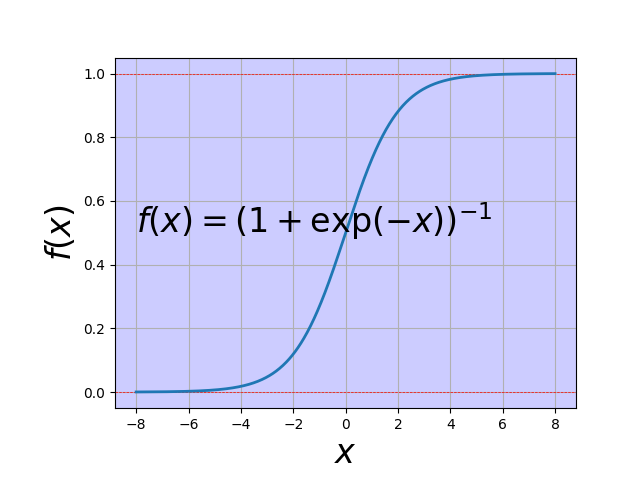
\includegraphics[width=8cm]{../plots/sigmoid.png} }}
	\subfloat[ReLU]{{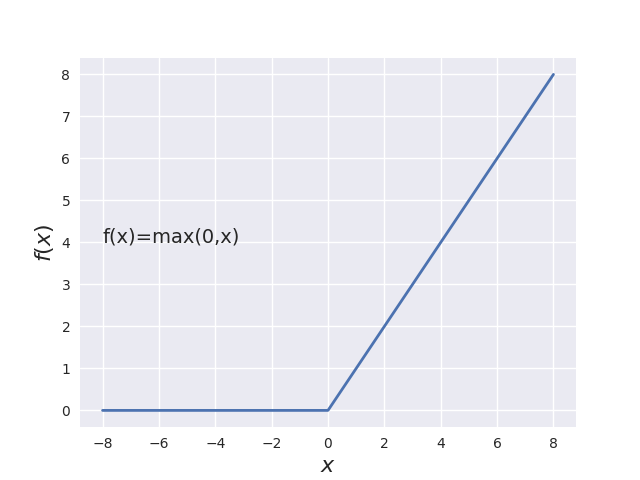
\includegraphics[width=8cm]{../plots/ReLU.png} }}\\
	
	\subfloat[Leaky ReLU]{{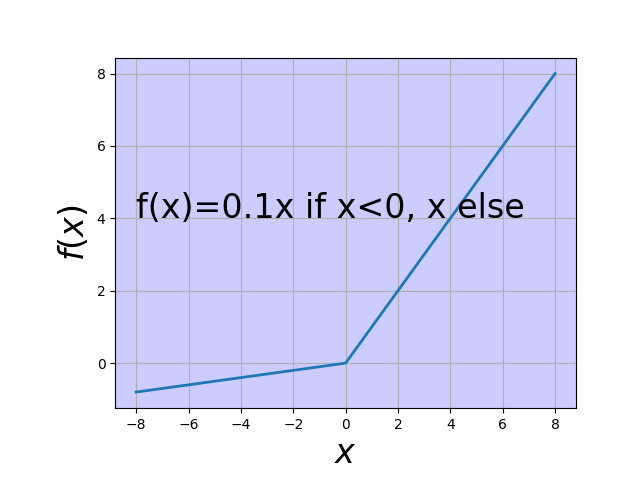
\includegraphics[width=8cm]{../plots/LeakyReLU.png} }}%
	\subfloat[ELU]{{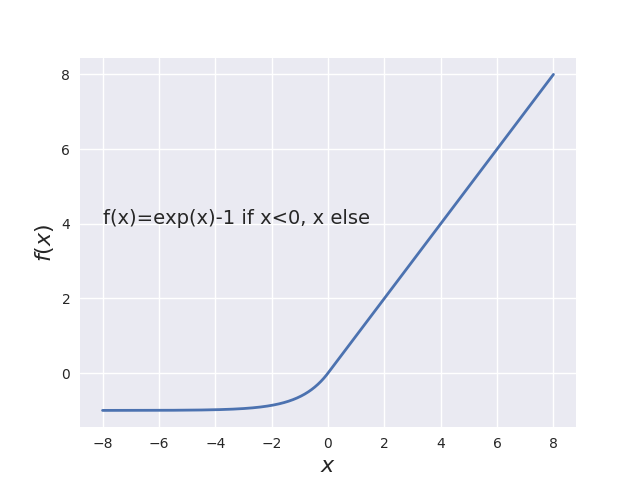
\includegraphics[width=8cm]{../plots/ELU.png} }}
	\caption{Some more or less popular activation functions}%
	\label{fig:activation_functions}%
\end{figure}
\fi

\subsubsection{Backward Propagation} \label{sec:backward}
Backward propagation is probably the most used technique for updating the weights, and is actually again based on equation (\ref{eq:w_update}). What differs, is the differentiation of the net input with respect to the weight, which gets more complex as we add more layers. For one hidden layer, we have two sets of weights, where the last layer is updated in a similar way as for a network without hidden layer, but the inputs are replaced with the values of the hidden nodes:
\begin{empheq}[box={\mybluebox[5pt]}]{align}
	w_{ij}^{(2)+}= w_{ij}^{(2)} - \eta\cdot[f(h_i^Tw_{ij})-y_j]^Th_i.
\end{empheq}
We recognize the first part as $\delta_{ok}$, such that
\begin{empheq}[box={\mybluebox[5pt]}]{equation}
	w_{ij}^{(1)+} = w_{ij}^{(1)} - \eta\cdot\sum_{k=1}^{O}\delta_{ok}\cdot w_{jk}^{(2)}\cdot f'(out_{hj})\cdot x_i
\end{empheq}
where we recall $\delta_{ok}$ as
\begin{equation*}
	\delta_{ok}=-(t_{ok}-out_{ok})\cdot f'(out_{ok}).
\end{equation*}
For more layers, the procedure is the same, but we keep on inserting the obtained outputs from various layers.

\subsubsection{Summary}
Since it will be quite a lot calculations, I will just express the results here, and move the calculations to Appendix B. The forward phase in a three-layer perceptron is
\begin{empheq}[box={\mybluebox[5pt]}]{align}
	net_{hi}&=\sum_jw_{ji}^{(1)}\cdot x_j\notag\\
	out_{hi}&=\text{f}(net_{hi})\notag\\
	\notag\\
	net_{ki}&=\sum_jw_{ji}^{(2)}\cdot out_{hj}\\
	out_{ki}&=\text{f}(net_{ki})\notag\\
	\notag\\
	net_{oi}&=\sum_jw_{ji}^{(3)}\cdot out_{kj}\notag\\
	out_{oi}&=\text{f}(net_{oi})\notag
\end{empheq}
which can easily be turned into vector form. The backward propagation follows from the two-layer example, and we get
\begin{empheq}[box={\mybluebox[5pt]}]{align}
	w_{ij}^{(3)}&=w_{ij}^{(3)}-\eta\cdot\delta_{oj}\cdot out_{ki}\notag\\
	\notag\\
	w_{ij}^{(2)}&=w_{ij}^{(2)}-\eta\sum_{k=1}^O\delta_{ok}\cdot w_{jk}^{(3)}\cdot f'(out_{kj})\cdot out_{hi}\notag\\
	\notag\\
	w_{ij}^{(1)}&=w_{ij}^{(1)}-\eta\sum_{k=1}^O\sum_{l=1}^K\delta_{ok}\cdot w_{lk}^{(3)}\cdot f'(out_{kl})\cdot w_{jl}^{(2)}f'(out_{hj})\cdot x_i\notag
\end{empheq}
where we again use the short hand 
\begin{equation*}
	\delta_{oj}=(t_j-out_{oj})\cdot f'(out_{oj}).
\end{equation*}
If we compare with the weight update formulas for the two-layer case, we recognize some obvious connections, and it is easy to imagine how we can construct a general weight update algorithm, no matter how many layers we have. 

Now over to the problem we want to solve using neural networks.


\section{Unsupervised Learning}
How can we train using unsupervised learning?

\subsection{Statistical foundation}
Bayesian statistics

\subsection{Boltzmann Machines}
Boltzmann Machines are based on the more primitive Hopfield network, where a system of nodes is set up which defines the system energy. Inspired by statistical mechanics, the probability of finding the system in a state of energy $E$ is given by
\begin{equation}
P=\exp(-E/kT)
\end{equation}
which is the Boltzmann distribution, hence the name Boltzmann machine. $k$ is known as Boltzmann's constant and $T$ is the system temperature, but henceforth they both will be avoided by scaling $E'=E/kT$. 

In the most general form, all nodes are connected to all other nodes, that is an unrestricted Boltzmann machine, see figure .. for illustration. 

INSERT FIGURE

In the same manner as in a Feed-forward Neural Network, we can directly multiply each node $s_i$ with its respective inner weights $w_{ij}$ and then with the opposite node $s_j$, which defines the system energy together with the bias contributions. This gives the energy
\begin{equation}
E=-\sum_{i=1}^N\sum_{j=i}^N s_iw_{ij}s_j - \sum_{i=1}^Ns_ib_i
\end{equation}
for a system of $N$ nodes, which is the so-called binary-binary network and the most basic architecture. During training, the weights are adjusted in order to maximize the probability...

\subsection{Restricted Boltzmann Machines}
When there is an unrestricted guy, a restricted guy must exist as well. 